\section{Experiments and Application}

%We evaluate MODEST across three tasks: shallow DoF rendering (Section 3.1), defocus deblurring (Section 3.2) mainly and 3D reconstruction (Section 3.3) as an exploratory demonstration of the dataset's broader utility. Scene 1 is used as the primary test case throughout due to its optical complexity. Extended visualizations , in depth analysis and explanation can be found in the supplementary

We evaluate MODEST across three tasks: shallow DoF rendering (Section~\ref{subsec:shallow_dof}) and defocus deblurring (Section~\ref{subsec:deblur}). Scene 1 is used as the primary test case throughout due to its optical complexity.


% \subsection{Practical Constraints on Ground-Truth Depth Capture}
% We considered acquiring dense per-pixel depth ground truth for our high-resolution (5472$\times$3648) indoor sequences. However, existing sensing technologies are not suitable for this scenario. Static terrestrial LiDAR scanners, such as FARO Focus X330 used in the ETH3D dataset \cite{Ohno2025UltraDenseLiDAR, schops2017eth3d}, can produce tens of millions of points per scan, but require long stationary captures ($\approx$ 9 minutes per scan) and multiple viewpoints to resolve occlusions. Such systems are bulky and unsuitable for dynamic or in-the-wild image acquisition. Moreover, LiDAR data exhibits systematic artifacts near occlusion boundaries and reflective or transparent surfaces, requiring heavy post-processing.

% Mobile multi-beam LiDAR units provide real-time scanning but are inherently sparse, with limited vertical resolution (tens of scan lines), making dense pixel-aligned supervision at 5k resolution infeasible.\cite{IntelRealSenseDepthQuality} Stereo and RGB-D cameras (e.g., Intel RealSense D435 and Intel RealSense D455) are limited by small stereo baselines and exhibit rapidly increasing depth error beyond 4–6 meters\cite{Rustler2025StereoDepth}. Under typical indoor conditions within 10 m, depth precision degrades significantly and produces noisy or incomplete depth maps. Active pattern-projection systems improve density but require controlled lighting and scene modification (e.g., surface painting), and fail on thin, specular, or transparent objects. Consequently, no commercially available system can simultaneously provide dense, high-accuracy, pixel-aligned depth maps for high-resolution natural indoor scenes within 10 meters. Therefore, reliable ground-truth depth was not feasible at acquisition time.

\subsection{Shallow DoF Rendering Models}\label{subsec:shallow_dof}

% To evaluate the generalization capabilities of shallow Depth-of-Field (DoF) rendering methods on the MODEST dataset, we benchmarked three representative state-of-the-art models: BokehMe~\cite{peng2022bokehme}, Dr.Bokeh~\cite{sheng2024dr}, and BokehDiff~\cite{zhu2025bokehdiff}. These models are evaluated on 100 images for each of five focal lengths  (\texttt{fl28}-\texttt{fl70}mm). The experiment assesses the model's ability to synthesize the blurred target image ($f/2.8$ being the widest aperture) using the sharp image ($f/22$ aperture) as all-in-focus input. From the quantitative results presented in Tab.~\ref{tab:deblur_dof_results}, BokehDiff exhibits the best overall performance balance across the dataset, achieving the highest PSNR ($19.88$ dB) and the best perceptual score (LPIPS, $0.3576$). However, a comparison with its previously reported results on the real-world EBB! Val294 dataset~\cite{ignatovebb} highlights $20\%$ degradation in PSNR, showing a significant challenge in optical generalization. We observe similar trends across all models; for example, Dr.Bokeh’s overall SSIM of $0.7861$ represents a performance degradation of approximately $20\%$ compared to its performance on its original paper dataset. To ensure a fair evaluation, we remain faithful to the original implementations by supplying all inputs required by each model, including all-in-focus references and associated depth maps where applicable. Despite receiving these inputs, these architectures rely on implicit learning of camera parameters; they attempt to internalize the relationship between focal length, focus plane distance, and aperture through training priors rather than utilizing explicit physical constraints. Our results indicate that this implicit approach is insufficient for cross-dataset generalization, as the models fail to adapt to the authentic optical characteristics of full-frame DSLR systems. Disentangled Performance Analysis. The systematic structure of MODEST allows us to analyze DoF performance across isolated optical variables. As evidenced in Tab.~\ref{tab:deblur_dof_results}, we observe a clear correlation between focal length and rendering error; for instance, PSNR typically degrades as the focal length increases from \texttt{fl28} to \texttt{fl70}, even when the aperture is held constant. This suggests that models struggle to scale their predicted Circle of Confusion (CoC) accurately as the field-of-view narrows and lens magnification increases. Because MODEST provides explicit focus plane and stereo-depth information, it reveals that SOTA models do not just "blur incorrectly", they fail to localize the focal region entirely, often resulting in "focus reversal" where the background is sharpened at the expense of the foreground.

% As illustrated with 3 examples in Figure~\ref{fig:dof}, the predictions produced by these state-of-the-art DoF rendering models vary considerably from the correct shallow depth-of-field captured by the camera. Unlike in real camera where blur transitions occur smoothly and at regions determined by the optical focus plane, the predicted images often exaggerate blur, misplace the focal region, or introduce depth-of-field that does not correspond to the actual scene geometry. Examples highlight large image portions getting blurred incorrectly, showing the models' inability to predict focus plane. Sometimes, models focus on background instead of foreground, effectively reversing focus order.

% These errors are closely tied to how existing DoF and bokeh-rendering methods are trained. Datasets such as EBB!~\cite{ignatovebb}, BLB~\cite{bokehme_blb}, and other monocular paired collections provide an input image and a target blurred image without any optical information linking the blur magnitude to lens parameters or scene geometry. Because each image is given as a single monocular view, no information about depth or focus plane is available. Further, the existing datasets feature very few optical combinations on focal length or aperture, so the amount of blur across images is very dataset-specific. As a result, models trained on such data learn correlations between appearance and "blur style" instead of learning physically grounded depth-of-field formation. This lack of structure prevents networks from understanding where the camera is focusing, how blur should change with distance, or how the circle of confusion is determined by aperture, focal length, and focus distance. Consequently, when evaluated on real camera captures, these models struggle to replicate authentic DoF behavior or perform consistently across scenes, focus settings, or geometric configurations.

% MODEST overcomes these limitations by offering a capture protocol explicitly designed for studying shallow depth of field under controlled but realistic conditions. Each scene contains stereo images at multiple focal lengths, and for every focal length we provide calibration and inference sets with systematically varied wide range of apertures. This structure ensures that the DoF relation with depth, focus distance, and aperture is explicit. High-resolution stereo from two identical full-frame Canon EOS 6D cameras preserve authentic optical characteristics such as bokeh shape, lens characteristics, and depth-dependent blur gradients-properties that synthetic datasets cannot reproduce faithfully. Together, these components create a well-structured training set and a rigorous testbed for DoF, defocus and deblur tasks.

\begin{figure*}[t]  % * makes it span both columns
    \centering
    \setlength{\abovecaptionskip}{2pt}  % reduce space above caption
    \setlength{\belowcaptionskip}{25pt}  % optional: reduce space below caption
    % \includegraphics[width=\textwidth]{imgs/cvpr_bokeh_comparison.pdf}  \\
    % \includegraphics[width=\textwidth]{imgs/cvpr_bokeh_comparison_1.pdf} \\
    % \includegraphics[width=\textwidth]{imgs/cvpr_bokeh_comparison_2.pdf}
    \includegraphics[width=\textwidth]{imgs/cvpr_dof_scene1_roi.pdf}  \\
    \includegraphics[width=\textwidth]{imgs/cvpr_dof_IMG_0636.pdf}    
    % scale to text width    
    \caption{Three shallow depth-of-field (DoF) rendering methods for two different scenes. Both examples are for focal length of 70mm, sharp input is F22.0 aperture, output target is F2.8 aperture.}
    \label{fig:dof}        
\end{figure*}

%To evaluate the generalization capability of shallow depth-of-field (DoF) rendering methods on MODEST, we benchmark three representative state-of-the-art models: BokehMe~\cite{peng2022bokehme}, Dr.Bokeh~\cite{sheng2024dr}, and Bokehlicious~\cite{seizinger2025bokehlicious}. Each model is evaluated on 100 images for five focal lengths (\texttt{fl28}–\texttt{fl70} mm). The task is to synthesize shallow DoF images at $f/2.8$ using the corresponding sharp all-in-focus image captured at $f/22$. The table Tab.~\ref{tab:dof_results} show that while Dr.Bokeh achieves the best average PSNR (20.22 dB) and LPIPS (0.3464), while Bokehlicious obtains the highest SSIM (0.7324) and BokehMe achieves the lowest MOR (1.85), all models exhibit significantly lower performance compared to their originally reported results on datasets such as EBB!~\cite{ignatovebb}. The observed performance drop of roughly $\sim20\%$ in PSNR and SSIM indicates a clear difficulty in generalizing to the authentic optical characteristics captured in MODEST.

To evaluate the generalization capability of shallow depth-of-field (DoF) rendering methods on MODEST, we benchmark three representative state-of-the-art models: BokehMe~\cite{peng2022bokehme}, Dr.Bokeh~\cite{sheng2024dr}, and Bokehlicious~\cite{seizinger2025bokehlicious}. Each model is evaluated on 100 images for five focal lengths (\texttt{fl28}–\texttt{fl70} mm). The task is to synthesize shallow DoF images at $f/2.8$ using the corresponding sharp all-in-focus image captured at $f/22$. The table Tab.~\ref{tab:dof_results} shows that while Dr.Bokeh achieves the best average PSNR (20.22 dB) and LPIPS (0.3464), Bokehlicious obtains the highest SSIM (0.7324) and BokehMe achieves the lowest MOR (1.85), all models exhibit significantly lower performance compared to their originally reported results on datasets such as EBB!~\cite{ignatovebb}. The observed performance drop of roughly $\sim20\%$ in PSNR and SSIM indicates a clear difficulty in generalizing to the authentic optical characteristics captured in MODEST.

The structured design of MODEST enables a disentangled analysis of DoF rendering across focal lengths and scene conditions. As shown in Tab.~\ref{tab:dof_results}, rendering accuracy consistently degrades as the focal length increases from \texttt{fl28} to \texttt{fl70}, even when the aperture remains fixed. This trend suggests that existing models struggle to scale the predicted Circle of Confusion (CoC) as magnification increases and the field of view narrows. Visual examples in Fig.~\ref{fig:dof} further illustrate these limitations. Unlike real cameras, where blur transitions occur smoothly around the optical focus plane, the predicted outputs often exaggerate blur, misplace the focal region, or produce inconsistent depth-of-field patterns. In several cases, the models incorrectly sharpen background regions while blurring foreground objects, effectively reversing the expected focus order.


\begin{table*}[!h]
\centering
\caption{
Quantitative evaluation of depth Of field methods across five focal lengths and the overall average. Higher PSNR/SSIM and lower LPIPS indicate better performance. \vspace{-10pt}}
\resizebox{\textwidth}{!}{
\begin{tabular}{l|c c c c c|c c c c c|c c c c c|c c c c}
\toprule
\multirow{2}{*}{\textbf{Method}} &
\multicolumn{5}{c|}{\textbf{PSNR} $\uparrow$} &
\multicolumn{5}{c|}{\textbf{SSIM} $\uparrow$} &
\multicolumn{5}{c|}{\textbf{LPIPS} $\downarrow$} &
\multicolumn{4}{c}{\textbf{Average}} \\
& fl28 & fl36 & fl45 & fl60 & fl70 &
fl28 & fl36 & fl45 & fl60 & fl70 &
fl28 & fl36 & fl45 & fl60 & fl70 &
PSNR$\uparrow$ & SSIM$\uparrow$ & LPIPS$\downarrow$ & MOR$\downarrow$\\
\midrule
\multicolumn{20}{l}{\textbf{Depth-of-Field (DoF) Methods}} \\
\midrule
% BokehDiff (`25)~\cite{zhu2025bokehdiff}&
% 22.03 & 21.98 & 19.33 & \textcolor{darkgreen}{18.40} & \textcolor{darkgreen}{17.66} &
% 0.6849 & 0.7031 & 0.6473 & 0.5691 & 0.5493 &
% 0.3387 & 0.3032 & \textcolor{darkgreen}{0.3014} & \textcolor{darkgreen}{0.3576} & 0.4830 &
% 19.88 & 0.6307 & 0.3576 \\
Bokehlicious (`25)~\cite{seizinger2025bokehlicious} &
22.48 & 22.63 & 18.80 & 18.01 & 17.50 & 0.7566 & 0.7787 & \textcolor{darkgreen}{0.7231} & \textcolor{darkgreen}{0.7141} & \textcolor{darkgreen}{0.7080} & 0.4842 & 0.4657 & 0.4891 & 0.4984 & 0.4737 & 19.60 & \textcolor{darkgreen}{0.7324} & 0.4831 &2.81 \\
Dr.Bokeh (`24)~\cite{sheng2024dr} &
\textcolor{darkgreen}{23.06} & \textcolor{darkgreen}{24.61} & \textcolor{darkgreen}{19.63} & 18.15 & 17.51 & \textcolor{darkgreen}{0.7747} & \textcolor{darkgreen}{0.8433} & 0.7215 & 0.6551 & 0.6437 & \textcolor{darkgreen}{0.2942} & \textcolor{darkgreen}{0.2343} & 0.3293 & 0.4007 & \textcolor{darkgreen}{0.4265} & \textcolor{darkgreen}{20.22} & 0.7175 & \textcolor{darkgreen}{0.3464} &2.01\\
BokehMe (`22)~\cite{peng2022bokehme} &
22.83 & 23.90 & 19.19 & 17.99 & 17.44 & 0.7702 & 0.8300 & 0.7133 & 0.6594 & 0.6551 & 0.3051 & 0.2717 & 0.3396 & 0.4107 & 0.4272 & 19.92 & 0.7165 & 0.3585 &\textcolor{darkgreen}{1.85}\\
\bottomrule
\end{tabular}}
\label{tab:dof_results}
\vspace{-10pt}
\end{table*}


These errors stem largely from how existing DoF rendering methods are trained. Popular datasets such as EBB!~\cite{ignatovebb} and BLB~\cite{bokehme_blb} provide monocular image pairs without explicit optical information linking blur magnitude to camera parameters or scene geometry. As a result, models learn correlations between appearance and blur style rather than the physical principles governing depth-of-field formation. In contrast, MODEST provides stereo imagery with known focus planes, multiple focal lengths, and systematically varied apertures, making the relationship between depth, aperture, and blur explicit. The use of two synchronized full-frame Canon EOS 6D cameras further preserves authentic lens characteristics such as realistic bokeh shapes and depth-dependent blur gradients. 



% \begin{figure*}[t]  % * makes it span both columns
%     \centering
%     \setlength{\abovecaptionskip}{2pt}  % reduce space above caption
%     \setlength{\belowcaptionskip}{25pt}  % optional: reduce space below caption
%     % \includegraphics[width=\textwidth]{imgs/cvpr_bokeh_comparison.pdf}  \\
%     % \includegraphics[width=\textwidth]{imgs/cvpr_bokeh_comparison_1.pdf} \\
%     % \includegraphics[width=\textwidth]{imgs/cvpr_bokeh_comparison_2.pdf}
%     \includegraphics[width=\textwidth]{imgs/cvpr_dof_scene1_roi.pdf}  \\
%     \includegraphics[width=\textwidth]{imgs/cvpr_dof_IMG_0636.pdf}    
%     % scale to text width    
%     \caption{Three shallow depth-of-field (DoF) rendering methods for two different scenes. Both examples are for focal length of 70mm, sharp input is F22.0 aperture, output target is F2.8 aperture.}
%     \label{fig:dof}        
% \end{figure*}


% \subsection{Deblurring models}\label{subsec:deblur}

% To study how well contemporary deblurring networks respond to aperture-driven blur, we evaluate three models: state-space model EVSSM~\cite{kong2025efficient} and two transformer-based models FFTformer~\cite{kong2023efficient} and Restormer~\cite{zamir2022restormer} on the MODEST dataset.  These models are evaluated on 100 images for each of five focal lengths  (\texttt{fl28}-\texttt{fl70}mm), using blurred inputs captured at $f/2.8$ aperture and sharp all-in-focus references at $f/22$ aperture. This setup enables us to examine the models’ behavior under structured optical blur that varies with focal length. We provide multiple deblurring illustrations in supplementary material due to space constraints.
% % add 2 defocus deblurring methods, do not remove existing ones.

% Across the focal-length groups, the results in Tab.~\ref{tab:dof_results} show that Restormer generally achieves stronger reconstructions than FFTformer. However, when contrasted with their performance on standard benchmarks, the models exhibit a substantial decline on MODEST. For instance, Restormer drops from roughly $32.9$~dB on GoPro dataset~\cite{nah2017deep} to $20.6$~dB on our dataset-a reduction of nearly $37\%$ in PSNR; while FFTformer~\cite{kong2023efficient} shows a similar decrease of about $40\%$. SSIM follows the same trend, with both models losing approximately $20\%$ relative to their originally reported values. These pronounced drops illustrate the difficulty current architectures face in handling aperture-produced optical blur and highlight the value of MODEST as a dataset for stress-testing deblurring models under controlled, optically grounded conditions.

% As shown in Fig , all deblurring methods appear to perform well and look similar when seen without zooming in, with VitDeblur showing slightly better results in zoomed-in views. Upon a closer examination reveals consistent failures across several challenging scenarios, like minute structural details, transparent materials, point light reflections on reflective surfaces, light sources and many other instances. These cases are analyzed in greater detail in the supplementary material.


\subsection{Deblurring Models}\label{subsec:deblur}

\begin{figure*}[t]  % * makes it span both columns
    \centering
    \setlength{\abovecaptionskip}{2pt}  % reduce space above caption
    \setlength{\belowcaptionskip}{25pt}  % optional: reduce space below caption
    % \includegraphics[width=\textwidth]{imgs/cvpr_bokeh_comparison.pdf}  \\
    % \includegraphics[width=\textwidth]{imgs/cvpr_bokeh_comparison_1.pdf} \\
    % \includegraphics[width=\textwidth]{imgs/cvpr_bokeh_comparison_2.pdf}
    \includegraphics[width=\textwidth]{imgs/cvpr_deblur_comparison_scene1_roi_1.pdf}  \\
    \includegraphics[width=\textwidth]{imgs/cvpr_deblur_comparison_scene1_roi.pdf}    
    % % scale to text width    
    % \caption{2 examples of focual length of 60mm and 70mm running inferene on 3 deblurring models , where the input was given as F2.8 Aperture and GT acting as F22.0 }

    \caption{Qualitative comparison of three deblurring models for focal lengths of 60\,mm and 70\,mm. The input images are captured at $f/2.8$ while the ground-truth images correspond to the sharp all-in-focus capture at $f/22$.}
    \label{fig:deblu}        
\end{figure*}

To evaluate aperture-induced defocus blur, we benchmark three recent defocus deblurring models: Restormer~\cite{zamir2022restormer}, ViTDeblur~\cite{li2022vitdeblur}, and NRKNet~\cite{quan2023neumann}. These methods are designed to recover sharp images from spatially varying defocus blur and therefore represent strong baselines for this task. For completeness, we additionally include two motion-deblurring architectures, EVSSM~\cite{kong2025efficient} and FFTformer~\cite{kong2023efficient}. These models were originally trained on motion-blur datasets and are not intended for defocus restoration; they are evaluated here only to assess how motion-trained networks generalize to optical defocus.

%Evaluation is performed on 100 images for each of five focal lengths (\texttt{fl28}–\texttt{fl70}). The blurred input corresponds to images captured at the widest aperture ($f/2.8$), while the reference images are the corresponding all-in-focus captures at $f/22$. This setup produces real, depth-dependent defocus blur generated by the camera optics rather than synthetic kernels. Quantitative results in Tab.~\ref{tab:deblur_results} show that the defocus-oriented methods consistently outperform the motion-deblurring models, although the overall performance remains modest. For instance, Restormer achieves an average PSNR of $20.6$,dB on MODEST, substantially lower than the $\sim32.9$,dB reported on the GoPro motion-blur benchmark~\cite{nah2017deep}, highlighting the gap between motion blur and optical defocus restoration.

Evaluation is performed on 100 images for each of five focal lengths (\texttt{fl28}–\texttt{fl70}). The blurred input corresponds to images captured at the widest aperture ($f/2.8$), while the reference images are the corresponding all-in-focus captures at $f/22$. This setup produces real, depth-dependent defocus blur generated by the camera optics rather than synthetic kernels. Quantitative results in Tab.~\ref{tab:deblur_results} show that the defocus-oriented methods consistently outperform the motion-deblurring models, although the overall performance remains modest. For instance, Restormer achieves an average PSNR of $20.6$dB on MODEST, substantially lower than the $\sim32.9$dB reported on the GoPro motion-blur benchmark~\cite{nah2017deep}, highlighting the gap between motion blur and optical defocus restoration.

Qualitative results in Fig.~\ref{fig:deblu} further illustrate the difficulty of the task. While most methods produce visually plausible outputs at a coarse scale, magnified regions reveal persistent artifacts around fine structures, reflective surfaces, transparent objects, and small light sources. These errors arise from the spatially varying and depth-dependent nature of defocus blur, which differs fundamentally from the blur models typically used during training. % Additional visualizations and failure cases are provided in the supplementary material.


% \begin{table*}[!h]
% \centering
% \caption{
% Quantitative evaluation of depth Of field methods across five focal lengths and the overall average. Higher PSNR/SSIM and lower LPIPS indicate better performance. \vspace{-10pt}}
% \resizebox{\textwidth}{!}{
% \begin{tabular}{l|c c c c c|c c c c c|c c c c c|c c c c}
% \toprule
% \multirow{2}{*}{\textbf{Method}} &
% \multicolumn{5}{c|}{\textbf{PSNR} $\uparrow$} &
% \multicolumn{5}{c|}{\textbf{SSIM} $\uparrow$} &
% \multicolumn{5}{c|}{\textbf{LPIPS} $\downarrow$} &
% \multicolumn{4}{c}{\textbf{Average}} \\
% & fl28 & fl36 & fl45 & fl60 & fl70 &
% fl28 & fl36 & fl45 & fl60 & fl70 &
% fl28 & fl36 & fl45 & fl60 & fl70 &
% PSNR$\uparrow$ & SSIM$\uparrow$ & LPIPS$\downarrow &MOR\downarrow$\\
% \midrule
% \multicolumn{20}{l}{\textbf{Depth-of-Field (DoF) Methods}} \\
% \midrule
% % BokehDiff (`25)~\cite{zhu2025bokehdiff}&
% % 22.03 & 21.98 & 19.33 & \textcolor{darkgreen}{18.40} & \textcolor{darkgreen}{17.66} &
% % 0.6849 & 0.7031 & 0.6473 & 0.5691 & 0.5493 &
% % 0.3387 & 0.3032 & \textcolor{darkgreen}{0.3014} & \textcolor{darkgreen}{0.3576} & 0.4830 &
% % 19.88 & 0.6307 & 0.3576 \\
% Bokehlicious (`25)~\cite{seizinger2025bokehlicious} &
% 22.48 & 22.63 & 18.80 & 18.01 & 17.50 & 0.7566 & 0.7787 & \textcolor{darkgreen}{0.7231} & \textcolor{darkgreen}{0.7141} & \textcolor{darkgreen}{0.7080} & 0.4842 & 0.4657 & 0.4891 & 0.4984 & 0.4737 & 19.60 & \textcolor{darkgreen}{0.7324} & 0.4831 &2.81 \\
% Dr.Bokeh (`24)~\cite{sheng2024dr} &
% \textcolor{darkgreen}{23.06} & \textcolor{darkgreen}{24.61} & \textcolor{darkgreen}{19.63} & 18.15 & 17.51 & \textcolor{darkgreen}{0.7747} & \textcolor{darkgreen}{0.8433} & 0.7215 & 0.6551 & 0.6437 & \textcolor{darkgreen}{0.2942} & \textcolor{darkgreen}{0.2343} & 0.3293 & 0.4007 & \textcolor{darkgreen}{0.4265} & \textcolor{darkgreen}{20.22} & 0.7175 & \textcolor{darkgreen}{0.3464} &2.01\\
% BokehMe (`22)~\cite{peng2022bokehme} &
% 22.83 & 23.90 & 19.19 & 17.99 & 17.44 & 0.7702 & 0.8300 & 0.7133 & 0.6594 & 0.6551 & 0.3051 & 0.2717 & 0.3396 & 0.4107 & 0.4272 & 19.92 & 0.7165 & 0.3585 &\textcolor{darkgreen}{1.85}\\
% \bottomrule
% \end{tabular}}
% \label{tab:dof_results}
% \vspace{-10pt}
% \end{table*}


\begin{table*}[!h]
\centering
\caption{
Quantitative evaluation of deblurring methods across five focal lengths and the overall average. Higher PSNR/SSIM and lower LPIPS indicate better performance. The table is structured into two deblurring sections (Defocus and Motion).\vspace{-10pt}}
\resizebox{\textwidth}{!}{
\begin{tabular}{l|c c c c c|c c c c c|c c c c c|c c c c}
\toprule
\multirow{2}{*}{\textbf{Method}} &
\multicolumn{5}{c|}{\textbf{PSNR} $\uparrow$} &
\multicolumn{5}{c|}{\textbf{SSIM} $\uparrow$} &
\multicolumn{5}{c|}{\textbf{LPIPS} $\downarrow$} &
\multicolumn{4}{c}{\textbf{Average}} \\
& fl28 & fl36 & fl45 & fl60 & fl70 &
fl28 & fl36 & fl45 & fl60 & fl70 &
fl28 & fl36 & fl45 & fl60 & fl70 &
PSNR$\uparrow$ & SSIM$\uparrow$ & LPIPS$\downarrow$ &MOR$\downarrow$\\
\midrule
\multicolumn{19}{l}{\textbf{Defocus Deblurring Methods}} \\
\midrule
Restormer (`22)~\cite{zamir2022restormer} &
\textcolor{darkgreen}{23.24} & 25.81 & 20.44 & 18.25 & 17.53 &
0.8052 & \textcolor{darkgreen}{0.8518} & \textcolor{darkgreen}{0.7731} & 0.7236 & 0.7084 &
0.0726 & 0.0500 & \textcolor{darkgreen}{0.1017} & \textcolor{darkgreen}{0.1522} & \textcolor{darkgreen}{0.1932} &
20.63 & 0.7653 & \textcolor{darkgreen}{0.1206} \\
ViTDeblur (`22)~\cite{li2022vitdeblur} &
23.15 & \textcolor{darkgreen}{25.87} & \textcolor{darkgreen}{20.59} & \textcolor{darkgreen}{18.30} & \textcolor{darkgreen}{17.60} & 
\textcolor{darkgreen}{0.8088} & 0.8507 & 0.7714 & \textcolor{darkgreen}{0.7261} & \textcolor{darkgreen}{0.7085} & 
0.0828 & 0.0651 & 0.1104 & 0.1602 & 0.2044 & 
\textcolor{darkgreen}{20.68} & \textcolor{darkgreen}{0.7660} & 0.1310 \\
NRKNet (`23)~\cite{quan2023neumann} &
23.01 & 25.78 & 19.99 & 18.02 & 17.48 & 
0.7966 & 0.8502 & 0.7553 & 0.7160 & 0.7059 & 
\textcolor{darkgreen}{0.0671} & \textcolor{darkgreen}{0.0416} & 0.1045 & 0.1600 & 0.2141 & 
20.42 & 0.7574 & 0.1254 \\

\midrule
\multicolumn{19}{l}{\textbf{Motion Deblurring Methods}} \\
\midrule
EVSSM (`25)~\cite{kong2025efficient} & 
22.64 & 23.61 & 18.76 & 17.03 & 16.55 & 
0.8089 & 0.8470 & 0.7573 & 0.7175 & 0.6996 & 
\textcolor{darkgreen}{0.0964} & \textcolor{darkgreen}{0.0795} & \textcolor{darkgreen}{0.1335} & \textcolor{darkgreen}{0.1889} & \textcolor{darkgreen}{0.2429} & 
19.34 & 0.7586 & \textcolor{darkgreen}{0.1557} \\
FFTformer (`23)~\cite{kong2023efficient} &
\textcolor{darkgreen}{23.44} & \textcolor{darkgreen}{24.78} & \textcolor{darkgreen}{19.58} & \textcolor{darkgreen}{17.44} & \textcolor{darkgreen}{16.97} &
\textcolor{darkgreen}{0.8175} & \textcolor{darkgreen}{0.8496} & \textcolor{darkgreen}{0.7695} & \textcolor{darkgreen}{0.7319} & \textcolor{darkgreen}{0.7129} &
0.1225 & 0.1094 & 0.1663 & 0.2326 & 0.2783 &
\textcolor{darkgreen}{20.03} & \textcolor{darkgreen}{0.7694} & 0.1898\\
\bottomrule
\end{tabular}}
\label{tab:deblur_results}
\vspace{-10pt}
\end{table*}

% \begin{figure*}[!t]  % * makes it span both columns
%     \centering
%     \setlength{\abovecaptionskip}{2pt}
%     \setlength{\belowcaptionskip}{2pt}    
%     \begin{subfigure}{\textwidth}
%     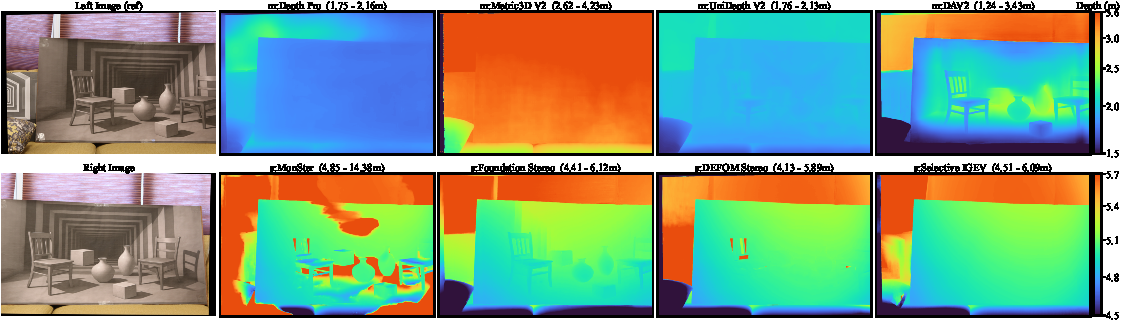
\includegraphics[width=\textwidth]{imgs/illusions_used_S6_16_visualization_frame_0.pdf}\vspace{-10pt}
%     \subcaption{\vspace{-16pt}}
%     \end{subfigure}
%     \begin{subfigure}{\textwidth}
%     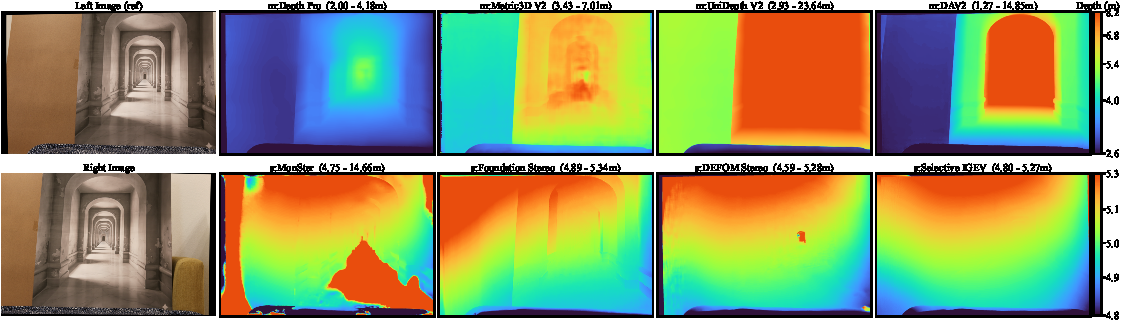
\includegraphics[width=\textwidth]{imgs/illusions_used_S6_10_visualization_frame_0.pdf}\vspace{-10pt}
%     \subcaption{\vspace{-16pt}}
%     \end{subfigure}
%     \begin{subfigure}{\textwidth}
%     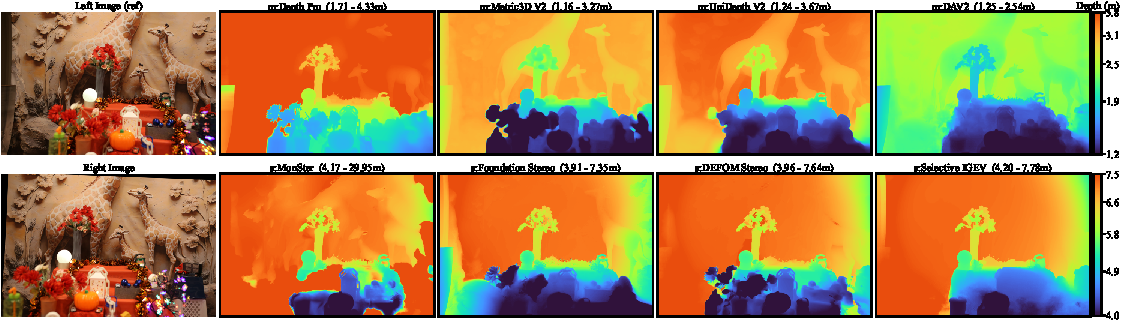
\includegraphics[width=\textwidth]{imgs/S9_f40_img_3901_visualization_frame_0.pdf}\vspace{-8pt}  
%     \end{subfigure}

%     \begin{subfigure}{\textwidth}
%     \begin{minipage}[t]{0.2\textwidth}
%         \centering
%         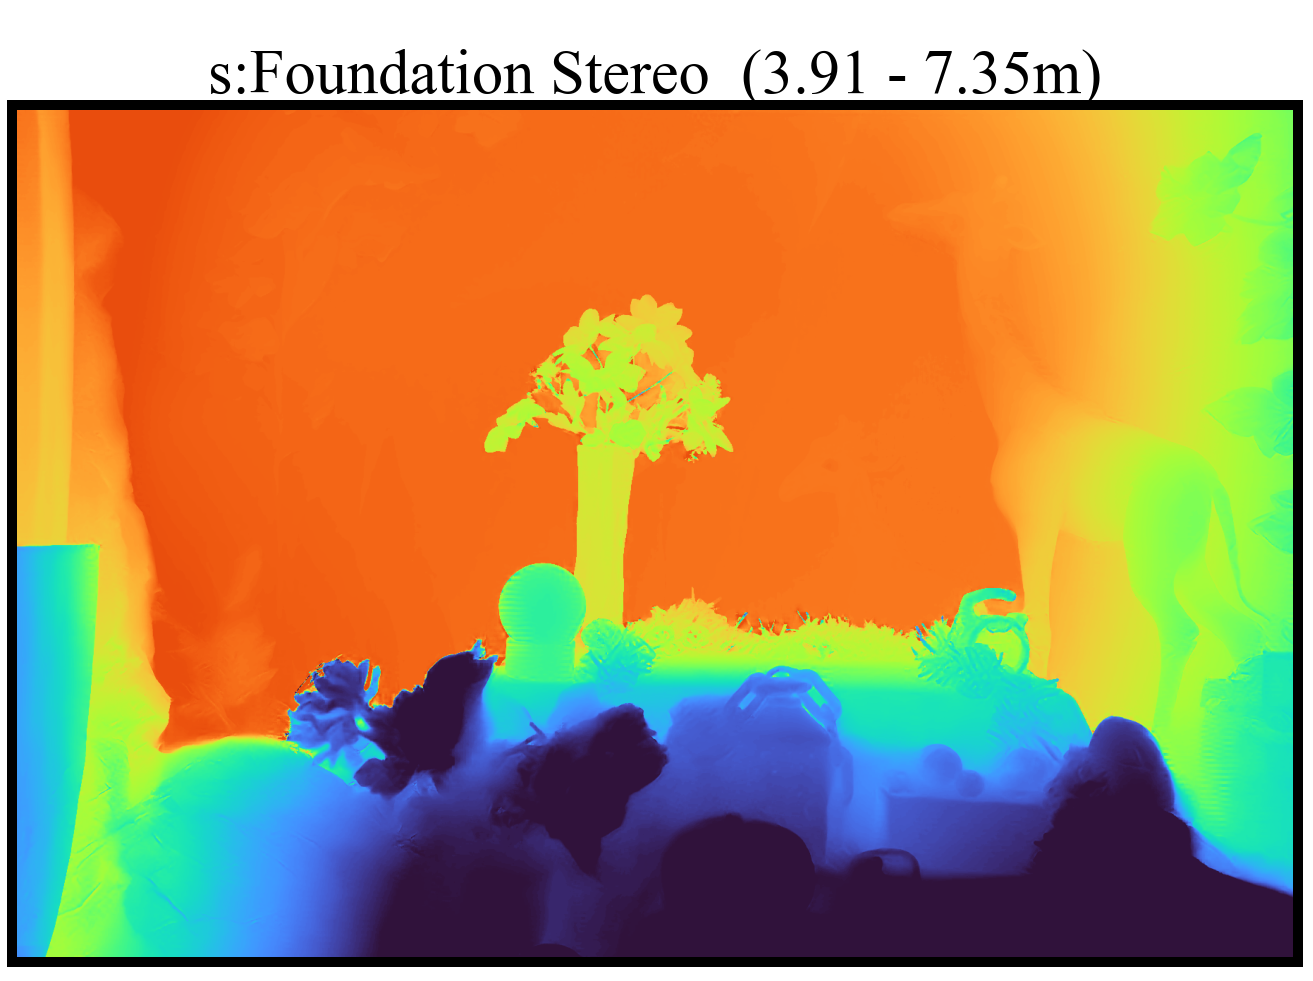
\includegraphics[width=\linewidth,height=0.68\linewidth]{imgs/S9_f40_img_3901_foundation.png}\vspace{-12pt}
%     \end{minipage}%
%     \hfill
%     \begin{minipage}[t]{0.8\textwidth}
%         \centering
%         \includegraphics[width=\linewidth]{imgs/error_maps_7.pdf}\vspace{-12pt}
%     \end{minipage}\vspace{-12pt}   
%     \subcaption{}
%     \end{subfigure}    

%     \caption{SOTA 4 monocular and 4 stereo depth estimation models are evaluated on 3 image pairs with optical illusions. The last row shows four error components for the Foundation Stereo~\cite{foundation} depth map, highlighting errors that are visually subtle but geometrically significant. Gradient error and planarity error $(\times 1e6)$ share a common colormap. All depth maps are produced in the left view. Monocular and stereo models are denoted by m: and s: prefixes respectively; depth ranges show ($5\text{–}95\%$ile).}
%     \label{fig:illusions}
% \end{figure*}






%\subsection{Multi-View Stereo and 3D Reconstruction}\label{subsec:mvs}

%\subsubsection{Classical MVS Limitations}
%We first attempted 3D reconstruction using classical multi-view stereo (MVS) pipelines such as COLMAP~\cite{colmap1,colmap2} and OpenMVS~\cite{openmvs}. While widely used, these geometry-driven approaches exhibit practical limitations on high-resolution indoor scenes. Patch-based stereo relies on photometric consistency and Lambertian reflectance assumptions; therefore reflective, transparent, or glossy materials (e.g., metal, acrylic, glass) introduce severe matching ambiguities and missing regions~\cite{pol_mvs2}. Low-texture or planar surfaces such as walls and cardboard also produce unstable depth estimates due to insufficient discriminative features~\cite{yang_mvs3}.

%From a computational perspective, dense reconstruction is expensive. A full reconstruction using 120 high-resolution views required more than 50\,GB of memory and several hours of runtime on an NVIDIA A100 GPU. Reducing iterations, sampling density, or image resolution accelerates computation but degrades geometric fidelity and depth consistency.

%In our experiments, classical pipelines often produced noisy or incomplete geometry. Smooth or specular surfaces yielded uncertain depth gradients, repeated textures caused mismatches, and thin structures such as wires or plant leaves were frequently unrecoverable. These observations highlight the sensitivity of traditional MVS to reflectance properties, texture availability, and triangulation geometry in realistic indoor scenes.

%\subsubsection{Learning-based Reconstruction}
%To explore modern alternatives, we evaluated a recent learning-based MVS model, MapAnything~\cite{keetha2025mapanything}. Unlike optimization-heavy pipelines such as COLMAP or OpenMVS, this transformer-based architecture predicts globally consistent geometry directly from multi-view images without explicit bundle adjustment or iterative stereo matching.

%The resulting point clouds demonstrate that the model can recover the primary scene structure, including surfaces, background geometry, and major objects, while maintaining spatial continuity across views. Compared to classical MVS, the reconstructions are typically denser and smoother, particularly in regions where traditional stereo struggles (e.g., low-texture or reflective surfaces). However, artifacts remain around thin structures, object boundaries, and specular regions. The model also occasionally interprets planar printed backdrops as volumetric structures, revealing ambiguities between appearance cues and true scene geometry.

%\subsubsection{Evaluation Protocol}
%Our dataset is designed as a diagnostic stress test for multi-view stereo and depth estimation methods rather than a benchmark with absolute ground truth. We therefore do not treat COLMAP reconstructions as reference geometry. Instead, methods are analyzed through downstream tasks such as depth-of-field rendering and defocus deblurring, which expose geometric inconsistencies. This protocol emphasizes identifying systematic failure modes rather than ranking methods against potentially biased reconstructions.

%\subsection{Neural 3D Representations (NeRF, GS)}\label{subsec:use_gs}

%Although 3D reconstruction is not the primary motivation of this work, the dataset can also support neural scene reconstruction approaches such as NeRF-style radiance fields and Gaussian Splatting (GS). The calibrated multi-view captures with varying focal lengths and apertures provide the geometric consistency and photometric diversity required for training and evaluating neural 3D representations.

%Both reconstructions produced using a learning-based MVS method and Gaussian Splatting via Splatter3R~\cite{smart2024splatt3r} recover coherent global structure but exhibit characteristic artifacts, including floating geometry near thin structures and inconsistencies where optical appearance cues conflict with true 3D layout. These observations suggest that MODEST can serve as a challenging dataset for evaluating next-generation neural reconstruction methods, particularly under complex indoor scenes and aperture-dependent image formation.

%Together, these evaluations demonstrate that MODEST exposes consistent failure modes in existing models that synthetic and low-resolution benchmarks do not, motivating the need for high-resolution, real-optics datasets in future training and evaluation pipelines






% \begin{figure}[t]
% \centering
% \includegraphics[width=0.49\linewidth,height=3.2cm]{imgs/MVS-demo.pdf}
% \hfill
% \includegraphics[width=0.49\linewidth,height=3.2cm]{imgs/GS2.pdf}

% \vspace{-3pt}
% \caption{Example 3D reconstructions on MODEST. 
% Left: learning-based multi-view stereo (MapAnything~\cite{keetha2025mapanything}). 
% Right: Gaussian Splatting using Splatter3R~\cite{smart2024splatt3r}. 
% These results illustrate that the dataset can also support neural 3D reconstruction, although this is not the main focus of the paper.}
% \label{fig:3d_scene}
% \vspace{-8pt}
% \end{figure}